\documentclass[11pt,a4paper]{report}
%\usepackage{showframe}
%\usepackage{listings,xcolor,beramono}
\usepackage{amssymb}
\usepackage{tikz}
\usetikzlibrary{shapes, arrows}
\usepackage{rotating}
\usepackage{caption}
\usepackage{cprotect}
\usepackage{multirow}
\usepackage{fancyvrb}
\usepackage{graphicx}
%\usepackage{menukeys}
\usepackage{subcaption}
\usepackage[
	hyperfootnotes=false
]{hyperref}
\usepackage[T1]{fontenc}
\usepackage{textcomp}
\usepackage{listings}
\renewcommand{\ttdefault}{pcr}
\lstset{
	language=HTML,
	basicstyle=\ttfamily\footnotesize,
	numbers=left,
	frame=bt,
	breaklines=true,
	showspaces=false,
	showstringspaces=false,
	captionpos=b,
	upquote=true,
	xleftmargin=5.0ex,
	xrightmargin=5.0ex,
	framexleftmargin=5.0ex,
	framexrightmargin=5.0ex,
	tabsize=4
}
\usepackage{calc}

\newcommand{\at}{\makeatletter @\makeatother}

\makeatletter
\newenvironment{btHighlight}[1][]
{\begingroup\tikzset{bt@Highlight@par/.style={#1}}\begin{lrbox}{\@tempboxa}}
{\end{lrbox}\bt@HL@box[bt@Highlight@par]{\@tempboxa}\endgroup}

\newcommand\btHL[1][]{%
  \begin{btHighlight}[#1]\bgroup\aftergroup\bt@HL@endenv%
}
\def\bt@HL@endenv{%
  \end{btHighlight}%   
  \egroup
}
\newcommand{\bt@HL@box}[2][]{%
  \tikz[#1]{%
    \pgfpathrectangle{\pgfpoint{1pt}{0pt}}{\pgfpoint{\wd #2}{\ht #2}}%
    \pgfusepath{use as bounding box}%
    \node[anchor=base west, fill=orange!30,outer sep=0pt,inner xsep=1pt, inner ysep=0pt, minimum height=\ht\strutbox+1pt,#1]{\raisebox{1pt}{\strut}\strut\usebox{#2}};
  }%
}
\makeatother

\lstdefinestyle{highlightable}{
    language=,
    moredelim=**[is][{\btHL[fill=black!18]}]{`}{`},
}

\newcommand{\Q}[2]{
	\label{#2}
	\marginpar{\textbf{Q#1.\begin{NoHyper}\ref{#2}\end{NoHyper} }}
}
\newcommand{\Qref}[2]{\hyperref[#2]{#1.\begin{NoHyper}\ref{#2}\end{NoHyper}}}
\newcounter{saveenumi}
\newcommand{\savei}{\setcounter{saveenumi}{\value{enumi}}}
\newcommand{\loadi}{\setcounter{enumi}{\value{saveenumi}}}
	
\newlength{\portraittextwidth}
\setlength{\portraittextwidth}{\textwidth}

\title{ELEC436 Portfolio}
\author{Christian Nassif-Haynes}
\date{16 June 2014}

\begin{document}
	\maketitle
	
	\chapter*{Preface}
	It is a software engineer's responsibility to keep her or his skill set up-to-date, be it by independent research or undertaking a formal course. Throughout my degree I have done the latter. In ELEC436, additional emphasis has been placed on the former, more self-guided form of learning which will be required during my career.
	
	To undertake this independent research most fruitfully, ELEC436 students familiarised themselves with the ACS-EA Joint Board software engineering competencies, then independently (of course, we could have asked for help along the way from Mike, our lecturer) satisfied those competencies which had not yet been covered. This document describes that research (Chapters~\ref{ch:distributed} and \ref{ch:networking}) in addition to work covered in class (all other Chapters).
	
	\tableofcontents
	
	\chapter{Distributed Computing} \label{ch:distributed}
	In this chapter I completed part of MIT's 6.824 2014 spring unit\footnote{\url{http://css.csail.mit.edu/6.824/2014/index.html}}. (My original intention was to use OpenCourseWare version of the unit, however the content was not new and relied on old software that I could not get to run on my machine.)
	
	
	\section{Introduction}
	Before talking in-depth about the work I did on distributed computing, it is wise to ask what the topic is about. I have knowledge on parallel computing, which is similar, from a previous unit (COMP226), so I will contrast the two here:
	\begin{itemize}
		\item In parallel computing, processors are connected to each other directly. Examples include multi-core CPUs or GPUs. In distributed computing, the processors are kept on separate machines connected via a network. One example is Folding\at home, in which work units are sent to each volunteer's personal computer via the Internet to be computed and returned to the server.
		\item In parallel computing, the same memory pool is usually shared by all processors, unlike in the distributed case where each CPU core gets its own.
	\end{itemize}
	
	\subsection{Setting Up}
	Version 1.2 of the Go programming language was required to complete the lab. I obtained a copy for Linux from \url{http://golang.org/doc/install}.
	
	\section{Lab 1}
	The link for the lab on MIT's website can be found here \url{http://css.csail.mit.edu/6.824/2014/labs/lab-1.html}.
	The full code I wrote can be found at the following repository: \url{https://bitbucket.org/DoxasticFox/lab-1/src/}
	
	\subsection{Overview}
	In this lab the aim was to implement the MapReduce algorithm. An overview of the algorithm is as follows~\cite{Dean:2008:MSD:1327452.1327492}:
	\begin{enumerate}
		\item The initial input is split up into pieces so that it can be distributed to workers.
		\item The workers are assigned pieces of the input by the master on which they execute a \verb=map= function. This function takes the input and expresses it as a set of key/value pairs.
		\item Sets of pairs from the \verb=map=ing step are forwarded to workers which execute a \verb=reduce= function on the sets.
		\item The pieces of output from the \verb=reduce= stage can be collated to form the final output.
	\end{enumerate}
	
	\subsection{Some Definitions}
	To discuss the lab in further detail, it is useful to define some associated terms first:
	\begin{description}
	\item[Mutex] Short for ``mutual exclusion''. In terms of go, this is a programming language construct designed to prevent sections of code from being executed, or resources from being accessed, at the same time. In other words, this prevents race conditions.
	\item[Race Condition] What occurs when a resource is accessed at the same time.
	\item[Go Channels] An alternative to mutexes which works by passing messages.
	\end{description}
	
	\subsection{Part I}
	In this part, the MapReduce algorithm was used to in a non-distributed manner (\verb=map= and \verb=reduce= jobs were not sent to workers) to calculate a word count for each word in the King James Bible. The code I wrote to achieve this can be found in the repository at \verb=src/main/go.wc=. The written code consists of three functions:
	\begin{itemize}
		\item \verb=NotLetter=---A helper function to segment the text into words.
		\item \verb=Map=---Takes a chunk of text as its argument and returns a list of pairs of the form $\langle w, 1 \rangle$, where $w$ is a word in the text.
		\item \verb=Reduce=---Takes a word $w$ and list of words $l$ and returns the number of times $w$ occurs in $l$.
	\end{itemize}
	
	In the MapReduce library implementation provided by MIT, the algorithm proceeds by splitting the Bible's text into pieces, calling \verb=DoMap= (the caller of \verb=Map=) on those pieces to produce intermediate files, calling \verb=DoReduce= (the caller of \verb=Reduce=) on those files, then merging the files produced to generate a list of word counts.
	
	\subsection{Part II}
	This part concerned the implementation of a master to allocate \verb=map= and \verb=reduce= jobs. What the \verb=Map= and \verb=Reduce= functions do are unimportant in this exercise. The implementation of this part can be found in the repository at \verb=src/mapreduce/master.go=. (Actually this is the code from part III.) The code I wrote is simply the \verb=RunMaster= function. An abridged version is shown here:
	\begin{lstlisting}[language=go]
func (mr *MapReduce) RunMaster() *list.List {
    mr.Workers = make(map[string]*WorkerInfo)
    mr.WorkersMtx = &sync.Mutex{}

    /* incessantly listen for new workers and add them
        to mr.Workers */
    go func() {
        for {
            var wi WorkerInfo
            // wait for worker address to come down channel
            wi.address = <-mr.registerChannel

            mr.WorkersMtx.Lock()
            mr.Workers[wi.address] = &wi
            mr.WorkersMtx.Unlock()
        }
    }()

    /* Map... */
    for i := 0; i < mr.nMap; {
        mr.WorkersMtx.Lock()
        for _, w := range mr.Workers {
            // try assigning reduce job. If successful do i++
            if i >= mr.nMap { break }
        }
        mr.WorkersMtx.Unlock()
    }

    /* ...reduce... */
    for i := 0; i < mr.nReduce; {
        mr.WorkersMtx.Lock()
        for _, w := range mr.Workers {
            // try assigning reduce job. If successful do i++
            if i >= mr.nReduce { break }
        }
        mr.WorkersMtx.Unlock()
    }
    return mr.KillWorkers() // ...termination.
}
	\end{lstlisting}
	
	\verb=mr.Workers= is a list of workers to which remote procedure calls (RPCs) may be made. The library provided by MIT made RPCs using Unix domain sockets. A mutex was used here as the goroutine (starting ``\verb=go func() {=...'') runs concurrently with the \verb=Map= and \verb=Reduce= functions, adding new workers to \verb=mr.Workers= when they are registered.
	
	\subsection{Part III}
	This part built on part II to handle the failure of workers. (In this case workers failed simply: they did not respond when assigned a job.) In the provided implementation, each worker had a set of properties associated it. To detect failures, a \verb=failed= property was added which was permanently set to \verb=true= if the worker did not respond. As well as this, the inner loops in the \verb=map= and \verb=reduce= stages of the algorithm were changed from, for example, this:
	\begin{lstlisting}[language=go]
for _, w := range mr.Workers {
    // try assigning reduce job. If successful do i++
    if i >= mr.nMap { break }
}
	\end{lstlisting}
	to this:
	\begin{lstlisting}[language=go]
for _, w := range mr.Workers {
    if w.failed { continue }
    // try assigning reduce job. If successful do i++
    // else w.failed = true
    if i >= mr.nMap { break }
}
	\end{lstlisting}
	
	\section{Lab 2}
	The link for the lab on MIT's website can be found here: \url{http://css.csail.mit.edu/6.824/2014/labs/lab-2.html}.
	The full code I wrote can be found at the following repository: \url{https://bitbucket.org/DoxasticFox/lab-2/src/}
	
	\subsection{Overview}
	In this lab a primary/backup replication service for a key/value database was set up. Clients who needed to access (read or write) a key/value pair were required to do so by making a RPC to a primary server, which was paired with a backup. Which server was the primary and which was the backup was decided by the \textit{viewservice}, which replied with numbered \textit{views} containing the primary and backups' Unix sockets.
	
	This lab spanned two weeks (one for each part) in the MIT course and provided hands-on knowledge of at-most-once semantics, mutexes, go channels and fault tolerance in distributed systems.
	
	\subsection{A Definition}
	To discuss the lab itself, it is useful to define the associated terminology:
	\begin{description}
	\item[At-most-once Semantics] An RPC is said to have this if the call executes exactly once or not at all. In order to implement this semantics duplicate RPC packets must be detected.
	\end{description}
	
	\subsection{Part A}
	In this part, the key/value service was given fault tolerance by adding a viewservice which designated the primary and backup roles for two subordinate servers. This was achieved by performing the following steps every time the viewservice's \verb|Ping| function in \verb|src/viewservice/server.go| was remotely called:
	\begin{enumerate}
		\item \textbf{Initialisation (}\verb|Ping|\textbf{ function variables)}---A snapshot of the current view was recorded along with the time of the \verb|Ping| RPC.
		\item \textbf{Initialisation (viewservice)}---It is checked if this is the viewservice's first received \verb|Ping|. If it is, the first pinging server is unconditionally set as the primary.
		\item \textbf{Detection of Primary's Acknowledgement}---An ``acknowledged'' flag is set if the primary server received the latest view. The view can only be updated if the primary has acknowledged the previous update. This rule prevents the viewservice from getting more than one view ahead of the key/value servers.
		\item \textbf{Update of the View}---Dead servers are removed, promotable servers are promoted, then the view number is incremented if the view changed.
	\end{enumerate}
	Note well that, to save resources, I should have written the code so that the view is updated every \verb|Tick|, however I did not have enough time to learn how to do so correctly.
	
	\subsection{Part B}
	In this part, fault tolerance was given to the key/value service: it was required to continue operating normally so long as there was never a time at which no primary or backup server was alive and; even if they were unable to access the viewservice momentarily.
	
	To help give fault tolerance, \verb|tick| in \verb|src/pbservice/server.go| was written so that the key/value pairs were sent to the (new) backup if it changed since the previous tick. The backup was kept up-to-date by forwarding key/value pairs to it when they were sent to the primary with a \verb|Put| RPC.
	
	A \verb|Commit| flag was given to \verb|common.go| to ensure at-most-once semantics:
	\begin{lstlisting}[language=go]
type PutArgs struct {
	Key string
	Value string
	DoHash bool // For PutHash
	Commit bool // Whether to commit changes to the database
}
	\end{lstlisting}
	In my implementation, to perform a put RPC, the client would send the datagram with the \verb|Commit| flag set to false, indicating that the key/value pair should not be stored. Upon receiving a reply, the client would resend with the flag toggled at which point the pair would be stored.
	
	In retrospect, at-most-once semantics could have been achieved better (that is with less network utilisation and more reliability) by using an acknowledgement and sequence number-style mechanism like in TCP (see Section~\ref{sec:tcp}). Nonetheless my server implementation still passed the unit tests.
	
	\chapter{Networking} \label{ch:networking}
	In many web browsers, pressing F11 enters full screen mode---something which I do from time to time. The keyboard's function keys are somewhat awkwardly placed however, making it easy to press an adjacent key. Inevitably, I have pressed F12 by mistake. In modern browsers (I use Firefox at the moment) doing so pops up a pane with curiously labelled tabs, including one which says ``Network'' as in Figure~\ref{fig:pressedf12figs}. One might wonder what a feature like this is doing in a program like a browser. Indeed, this common, inconspicuous feature has the ability to evoke a substantial line of questioning.
	
	In this chapter I aim to satisfy some of those more salient questions that arise as I experiment with freely available networking-related programs.
	
	\section{How to Use This Chapter}
	In the margin I have included numbers for the many questions that arise, according to the section they appear under, and in the order which they are asked. For the remainder of this chapter, when I make reference to a question without mentioning the section number it is understood that I am talking about the question in the same section it is referenced. 
	
	\section{Exploring Firefox's Developer Tools}
	A few curious features and questions on them can be noted about Figure~\ref{fig:pressedf12reloaded}:
	\begin{enumerate}
		\item What does each row represent? \Q{2}{enum:row}
		\item Why does each row have a triangle or circle? \Q{2}{enum:tricirc}
		\item The ``Method'' column says \textbf{GET} a lot. What does that mean? \Q{2}{enum:get}
		\savei
	\end{enumerate}
	\begin{figure}
		\centering
		\begin{subfigure}{\textwidth}
			\includegraphics[width=\textwidth]{pressedf12.png}
			\caption{I am told I can ``perform a request or reload the page to see detailed information about network activity''.}
			\label{fig:pressedf12}
		\end{subfigure} \\
		\vspace{0.5cm}
		\begin{subfigure}{\textwidth}
			\includegraphics[width=\textwidth]{pressedf12reloaded.png}
			\caption{What I see when I reload the page.}
			\label{fig:pressedf12reloaded}
		\end{subfigure}
		\caption{The Network tab under Firefox's Developer Tools when visiting \url{http://mq.edu.au}.}
		\label{fig:pressedf12figs}
	\end{figure}
	The answer to Question~\ref{enum:row} is not of prime importance but helps to contextualise answers to other questions, so I will provide it briefly here. Taking a look at the source code for site shown in Figure~\ref{fig:pressedf12figs} (by right-clicking the page and clicking ``View Page Source''), it can be seen that the ``File'' and ``Domain'' columns show URLs that appear in the source code. For example, the file \verb|Jubilee-988x248-v3.jpg| appears in Figure~\ref{fig:pressedf12reloaded} because it is mentioned at line 302 in the source. (A snippet from it is shown as Listing~\ref{li:mq302}.) Each URL in the source is, ostensibly, a resource which must be \textit{requested} from a web server in order to load the web page in full. This leads to a question which might be better than that in Question~\ref{enum:row}:
	\begin{enumerate}
		\loadi
		\item What is a request and what does my computer send and receive when my browser makes one? \Q{2}{enum:request}
		\savei
	\end{enumerate}
	
	\begin{figure}
	\begin{lstlisting}[firstnumber=296, xleftmargin=6.3ex, framexleftmargin=6.3ex, caption=A code snippet showing the source for the home page of Macquarie University., label=li:mq302]
        <div class="next-btn"></div>
      </div>
      <div class="thumbnails">
        <ul>
        <li><a href="mq_templates/corporate/homepage_banner_rotator/images/2014/Tokyo-MY-v2-homepage998x248banner.jpg"></a><a href="http://mq.edu.au/courses/areas_of_study/#ac=mid-year2014_tokyo_creative" onclick="_gaq.push(['rollup._trackEvent', 'MQ Homepage', 'banner', 'Tokyo Creative']);"></a></li>
        <li><a href="mq_templates/corporate/homepage_banner_rotator/images/2014/Accept-offer-apr2014-998x248.jpg"></a><a href="http://students.mq.edu.au/student_admin/enrolmentguide/acceptyouroffer" onclick="_gaq.push(['rollup._trackEvent', 'MQ Homepage', 'banner', 'Accept your offer']);"></a></li>
          <li><a href="mq_templates/corporate/homepage_banner_rotator/images/2014/Jubilee-998x248-v3.jpg"></a><a href="http://jubilee.mq.edu.au/homepage/1" onclick="_gaq.push(['rollup._trackEvent', 'MQ Homepage', 'banner', 'Jubilee']);"></a></li>
          <li> <a href="mq_templates/corporate/homepage_banner_rotator/images/2014/QS5star-998x248.jpg"></a> <a href="http://www.mq.edu.au/future_students/international/why_choose_macquarie/our_reputation/university_rankings/" onclick="javascript: _gaq.push(['rollup._trackEvent', 'MQ Homepage', 'banner', 'QS 5 star']);"></a></li>
        </ul>
      </div>
    </div>
  </div>
</div>
<!-- endMain Gallery container --> 
	\end{lstlisting}
	\end{figure}
	
	Clicking on a row gives a hint towards the answer to Question~\ref{enum:tricirc}. Upon doing so the pane pictured in Figure~\ref{fig:tricirc} appears, showing that the triangle represents the \verb|304 Not Modified| status code and the circle, \verb|200 OK|. What do these codes mean? Searching Google for ``304'' returns The Internet Engineering Task Force's (IETF) RFC 2616~\cite{http-rfc} as the first result, in which these status codes were officially defined. From this I can conclude that:
	\begin{itemize}
		\item Status codes (like \verb|304| and \verb|200|), requests and GET methods are part of the Hypertext Transfer Protocol (HTTP).
		\item HTTP is a text-based protocol.
		\item This line of questioning is so far leading to an insight of networks which is abstracted away from, for example, how data find their way from one computer to the next.\footnote{This is because the explanation so far has been centered on HTTP, which operates at the application level~\cite[Section~1.1]{http-rfc}.} %QUESTIONQUESTIONQUESTION
		%how data finds its way from one computer to the next
		%QUESTIONQUESTIONQUESTION
	\end{itemize}
	
	\begin{figure}
		\includegraphics[width=\textwidth]{tricirc.png}
		\caption{The HTTP headers for a request.}
		\label{fig:tricirc}
	\end{figure}
	
	Additionally, in regards to Question~\ref{enum:get}, RFC 2616 states fairly plainly that:
	\begin{itemize}
		\item ``The GET method means retrieve whatever information ... is identified by the Request-URI\footnote{This is roughly equivalent to a URL.}''~\cite[Section~9.3]{http-rfc}.
	\end{itemize}
	
	Interestingly, knowing that HTTP is a text-based protocol and the form of GET requests, I should be able to retrieve a web page using only the \verb|telnet| program. \url{http://www.w3.org/pub/WWW/TheProject.html} is given in RFC 2616 as an example~\cite[Section~5.1.2]{http-rfc}. If a user was to type this URL into a browser, the following lines would be sent, as text, to the server which hosts it:
	\begin{lstlisting}[style=highlightable, frame=none, numbers=none, xleftmargin=0ex, xrightmargin=0ex]
GET /pub/WWW/TheProject.html HTTP/1.1<CRLF>
Host: www.w3.org<CRLF>
<CRLF>
	\end{lstlisting}
	(Here \verb|<CRLF>| is used to denote a carriage return followed by a linefeed.) These two lines form a \textit{request}. Using this example I can GET \begin{NoHyper}\url{http://mq.edu.au}\end{NoHyper} via the terminal as shown in Listing~\ref{li:telnet}.
	Here the three lines ending with \verb|<CRLF>| (the return key) are my input. I set \verb|telnet| to use port 80 as RFC 2616 mentions that it is the default port, citing Reynolds and Postel~\cite{ports}. I would like to know:
	\begin{enumerate}
		\loadi
		\item What is a port? \Q{2}{enum:port}
		\savei
	\end{enumerate}
	The RFC also mentions that ``HTTP communication usually takes place over TCP/IP connections'':
	\begin{enumerate}
		\loadi
		\item What is TCP/IP (or, for that matter, either one)? \Q{2}{enum:tcpip}
		\savei
	\end{enumerate}
	
	\begin{figure}
	\begin{lstlisting}[language=]
christian@christian-pc ~ $ telnet mq.edu.au 80<CRLF>
Trying 137.111.223.158...
Connected to mq.edu.au.
Escape character is '^]'.
GET / http/1.1<CRLF>
Host: mq.edu.au<CRLF>
<CRLF>
HTTP/1.1 200 OK
Date: Mon, 12 May 2014 13:21:18 GMT
Server: Apache
Cache-Control: max-age=7200, proxy-revalidate
Expires: Mon, 12 May 2014 15:21:18 GMT
Vary: Accept-Encoding,User-Agent
Transfer-Encoding: chunked
Content-Type: text/html

4b7d
<!DOCTYPE html>
<html xmlns="http://www.w3.org/1999/xhtml" lang="en" xml:lang=
"en">
	\end{lstlisting}
	\begin{center}
		\textit{The response body (HTML code) has been omitted for brevity.}
	\end{center}
\begin{lstlisting}[language=, firstnumber=21, caption=Performing a HTTP request in telnet., label=li:telnet]
</html>

0



Connection closed by foreign host.
	\end{lstlisting}
	\end{figure}
	
	After all this, I have addressed Question~\ref{enum:request} in part, but the explanation so far is too high-level to be satisfying. Additionally, I noticed that \verb|telnet| has found the IP address for \url{mq.edu.au}, but:
	\begin{enumerate}
		\loadi
		\item How did \verb|telnet| find the IP address? \Q{2}{enum:howfindip}
		\item Why is it necessary to find it in the first place? \Q{2}{enum:whyfindip}
		\savei
	\end{enumerate}
	Moreover, now that I have seen some HTTP message text, I wonder:
	\begin{enumerate}
		\loadi
		\item Why does the response in Listing~\ref{li:telnet} appear to have sections (lines 8-16, lines 18-26)? \Q{2}{enum:sections}
		\savei
	\end{enumerate}
	
	Turning again to RFC 2616, I have my answer to Question~\ref{enum:sections}~\cite[Section~4]{http-rfc}. The three main sections shown in Listing~\ref{li:telnet} are:

	\begin{description}
		\setlength\labelsep{0.4cm}
		\item[Request {\rm (lines 5-7)}] \textit{As above}. Headers (additional information about the request) may be included, but lines 5 and 6 are mandatory.
		\item[Status-line {\rm and} response message headers {\rm (lines 8-16)}] The first line in this section is the status-line. It gives a HTTP status code like the ones I noted earlier. The subsequent lines are the response message headers, which contain any additional information about the response which cannot be placed in the status-line (e.g. things like the age of the requested resource and how long the client should cache it).
		\item[Response message body {\rm (lines 17-26)}] In this case, the message body is simply the HTML code of the requested page, however other media like images may be sent instead.
	\end{description}
	
	It should be noted that lines 17 and 23 are not HTML because the server is using chunked encoding\footnote{Initially I thought they were not HTML because the encoding of the message sent by the server did not match the encoding used in my terminal.}. These lines are the size of the chunks~\cite[Section~3.6.1]{http-rfc} that the client should expect. The last chunk (line 23 here) is necessarily of size zero.
	
	\section{What is ``Underneath'' HTTP? (The TCP Section)} \label{sec:tcp}
	In the previous section I asked some foundational questions about networks and found upon answering some that browsers access web pages by performing HTTP requests. Continuing along this line I found that generally more than one request is performed and usually by the GET method. The response to the request is sent back as text which includes not only the requested file, but metadata like status codes and headers as well. While learning of this, Questions~\Qref{2}{enum:port}, \Qref{2}{enum:tcpip}, \Qref{2}{enum:howfindip} and \Qref{2}{enum:whyfindip} arose, but were left open.
	
	To answer Question~\Qref{2}{enum:tcpip}, I turned to IETF's website again. Searching for ``TCP/IP'' conveniently returns RFC 1180, ``A TCP/IP Tutorial''~\cite{tcpip-tute}. Now, in Section 2, ``TCP/IP'' has been given the unfortunately vague definition of ``anything and everything related to the specific protocols of TCP and IP''. Fortunately, the situation is elucidated somewhat by Section 2.1, which gives the diagram in Figure~\ref{fig:tcpiporiginal}, showing common Internet protocols, in relation to each other, as a hierarchy. In particular it shows that TCP works ``over the top of'' IP. This diagram raises obvious questions which I will address later:
	\begin{enumerate}
		\item What is ARP? \Q{3}{enum:arp}
		\item How does Ethernet work? \Q{3}{enum:ethernet}
	\end{enumerate}
	
	\begin{figure}
		\centering
		\begin{subfigure}[t]{0.48\textwidth}
			\centering
			\begin{BVerbatim}[baselinestretch=0]
--------------------------
|                        |
|  network applications  |
|                        |
|... \ | /  ..  \ | / ...|
|    -----      -----    |
|    |TCP|      |UDP|    |
|    -----      -----    |
|        \      /        |
|        --------        |
|        |  IP  |        |
| -----  -*------        |
| |ARP|   |              |
| -----   |              |
|     \   |              |
|     ------             |
|     |ENET|             |
|     ---@--             |
---------|----------------
         |
    -----o-------------
           Ethernet Cable
			\end{BVerbatim}
			\caption{The original ASCII diagram from RFC 1180. The layout has been slightly modified here.}
			\label{fig:tcpiporiginal}
		\end{subfigure}~~
		\begin{subfigure}[t]{0.48\textwidth}
			\centering
			\begin{BVerbatim}[baselinestretch=0]
--------------------------
|     ------             |
|     |HTTP|             |
|     ------             |
|       |                |
|     -----              |
|     |TCP|              |
|     -----              |
|         \              |
|         --------       |
|         |  IP  |       |
|  -----  -*------       |
|  |ARP|   |             |
|  -----   |             |
|      \   |             |
|      ------            |
|      |ENET|            |
|      ---@--            |
----------|---------------
          |
     -----o-------------
            Ethernet Cable
			\end{BVerbatim}
			\caption{The diagram modified to show the place of HTTP (and the scope of this chapter).}
			\label{fig:tcpipmodified}
		\end{subfigure}
		\caption{Schematics showing a hierarchy of commonplace protocols though which data travel. The lines represent the flow of data, the asterisk an IP address, the ampersand an Ethernet (MAC) address and the ``o'' the transceiver (which converts electrical signals to Ethernet frames and vice versa). The boxes represent parts of the network which process data. ``ENET'' is one part which processes Ethernet frames.}
		\label{fig:tcpip}
		% (MAC)
		% ``ENET'' is one part which processes Ethernet frames.
	\end{figure}
	
	Now that I have the diagram in Figure~\ref{fig:tcpiporiginal} I can place HTTP at the top of the entire stack, at the application-level. Additionally, I have an overview of common network protocols in the hierarchy so that I can deal with TCP and IP separately. I will start with the former as it is the next lowest in the hierarchy after HTTP. RFC 793 gives the purpose of TCP along with an overview of its operation~\cite{tcp}. A summary of TCPs basic functions is as follows:
	\begin{itemize}
		\item \textbf{Basic data transfer}---TCP is able to be used to transfer a continuous stream of octets (bytes) via the Internet by grouping them into \textit{segments}.
		\item \textbf{Reliability}---TCP is able to deal with segments which are damaged, lost, duplicated or delivered out of order. Damage is dealt with by giving each segment a checksum. The remaining issues are dealt with by giving segments ACK and sequence numbers which count the number of octets transmitted. The receiver must correctly ACKnowledge each sent segment within a timeout period, else it is resent.
		\item \textbf{Flow control}---Using TCP, the receiver can set the maximum allowed number of octets sent without replying with an ACK. This is known as the \textit{window}.
		\item \textbf{Multiplexing}---By providing a set of ports to each host\footnote{This is roughly the same as a computer or some other network device.} TCP allows that host to use or provide multiple services at the same address. For example, in principle it is possible for the host at the single address, \url{mq.edu.au} to be running two services,  \verb|telnet| and the Macquarie University website, by having the former on port 23 and the latter on 80. (This answers Question~\Qref{2}{enum:port} directly!)
	\end{itemize}
	Figure~\ref{fig:tcpheader} shows the parts of the TCP header which store the aforementioned sequence numbers and other fields~\cite[Section 3.1]{tcp}.

	\begin{sidewaysfigure}
		\begin{tabular}{r|c|c|c|c|c|c|c|c|c|c|c|c|c|c|c|c|c|c|c|c|c|c|c|c|c|c|c|c|c|c|c|c|}
		\cline{2-33}
       & \multicolumn{8}{c|}{0}                                                                         & \multicolumn{8}{c|}{1}                                         & \multicolumn{8}{c|}{2}        & \multicolumn{8}{c|}{4}        \\ \cline{2-33} 
       & \multicolumn{1}{l|}{0} & 1 & 2 & 3 & 4            & 5            & 6            & 7            & 0            & 1           & 2   & 3   & 4   & 5   & 6   & 7   & 0 & 1 & 2 & 3 & 4 & 5 & 6 & 7 & 0 & 1 & 2 & 3 & 4 & 5 & 6 & 7 \\ \cline{2-33} 
		0       & \multicolumn{16}{c|}{Source Port}                                                                                                                               & \multicolumn{16}{c|}{Destination Port}                        \\ \cline{2-33} 
		32      & \multicolumn{32}{c|}{Sequence Number}                                                                                                                                                                                           \\ \cline{2-33} 
		64      & \multicolumn{32}{c|}{ACK Number}                                                                                                                                                                                                \\ \cline{2-33} 
		96      & \multicolumn{4}{c|}{Data Offset}   & \multicolumn{6}{c|}{\begin{tabular}[c]{@{}c@{}}Reserved for\\ Future Use\end{tabular}} & \multicolumn{6}{c|}{Control Bits} & \multicolumn{16}{c|}{Window Size}                             \\ \cline{2-33} 
		128     & \multicolumn{16}{c|}{Checksum}                                                                                                                                  & \multicolumn{16}{c|}{Urgent Pointer}                          \\ \cline{2-33} 
		160     & \multicolumn{32}{c|}{Options (Padded to 4-byte Boundary)}                                                                                                                                                                       \\ \cline{2-33} 
		160-480 & \multicolumn{32}{c|}{\multirow{2}{*}{Data}}                                                                                                                                                                                     \\
		...     & \multicolumn{32}{c|}{}                                                                                                                                                                                                          \\ \cline{2-33} 
		\end{tabular}
		\captionsetup{width=\portraittextwidth}
		\caption{The TCP packet format as defined in RFC 793. The numbers along the top row are the byte and bit numbers. Those along the left side are also for bits. Notice that the data can start \textit{between} bits 160-480 because the options section is of variable size. The payload (data) \textit{length} is similarly variable.}
		\label{fig:tcpheader}
	\end{sidewaysfigure}
		
	To make this concrete I have performed the same GET request as in the previous section of this chapter while running Wireshark, a segment analyser, to view the TCP segments. Figure~\ref{fig:wireshark1} shows the Wireshark window after having performed the request. In particular, in Figure~\ref{fig:wireshark2}, I can now see firsthand the way in which the segments are ACKed:
	\begin{itemize}
		\item Packet 1---The connection with the server (137.111.223.158) is established by sending a SYN segment. The ACK number does not matter as there is nothing for the client to acknowledge. Notice that although the sequence number is shown as zero, this is not the way it appears in the segment. Wireshark only shows the starting number as zero for readability.
		\item Packet 2---The server ACKnowledges the first SYN segment by taking the previously sent sequence number and incrementing it by one. Because the server has not previously sent anything in this connection, it sends a sequence number of zero.
		\item Packet 3---The client sends a segment with a sequence number of one indicating the SYN it sent just before. It also ACKnowledges the SYN by taking the sequence number sent with it, incrementing it and sending it as an ACK.
	\end{itemize}
	The client and server continue to communicate like this throughout the duration of the connection, only, just like SYNs have a ``weight'' of one, segments containing data are weighted by their length. Once the connection closes, the systems which were involved can free resources associated with maintaining it.
	
	As well as the ACK and sequence numbers, Wireshark can be used to show the TCP segment as binary\footnote{Wireshark does not show the output exactly as is done here. The formatting has been changed for easy comparison with Figure~\ref{fig:tcpheader}.}. The following is the first 44 bytes of frame 22 from Figure~\ref{fig:wireshark1}:
	{
		\setlength\topsep{0pt}
		\setlength\parskip{0pt}
		\begin{center}
		\begin{minipage}{0.7501\textwidth}
		\begin{lstlisting}[style=highlightable, frame=none, numbers=none, xleftmargin=0ex, xrightmargin=0ex]
0000000: 00000000 01010000 `11000001 11111001`  .P..
0000032: 01001001 10000111 01010101 00101110  I.U.
0000064: `00000110 00000111 10000010 00111110`  ...>
0000096: 1000`0000 00`010000 `00000000 00101110`  ....
0000128: 11101000 01010001 `00000000 00000000`  .Q..
0000160: 00000001 00000001 00001000 00001010  ....
0000192: 11010101 10011101 10101110 11101010  ....
0000224: 00001100 11100101 00100111 10111011  ..'.
0000256: `01001000 01010100 01010100 01010000`  HTTP
0000288: `00101111 00110001 00101110 00110001`  /1.1
0000320: `00100000 00110010 00110000 00110000`   200
		\end{lstlisting}
		\end{minipage}
		\end{center}
	}\noindent
	The left-most column shows the bit numbers. Alternating grey and white has been used here to show field boundaries. (Compare this to Figure~\ref{fig:tcpheader}). Binary conversions for some fields are as shown here:
	\begin{itemize}
		\item Source port: $00000000\;01010000_2 = 80_{10}$
		\item Destination port: $11000001\;11111001_2 = 49,\!657_{10}$
		\item Sequence number: Notice that as this is the 1\textsuperscript{st} (relative) sequence number, the 0\textsuperscript{th} must have been $1,\!233,\!605,\!933_{10}$. The conversion is as follows: $01001001\;10000111\;01010101\;00101110_2 = 1,\!233,\!605,\!934_{10}$.
		\item ACK number: $\!00000110\,00000111\,10000010\,00111110_2 = 101,\!155,\!390_{10}$
	\end{itemize}
	Notice that the options field is 12 bytes long in this case. The data field, which contains some of the HTTP text, begins at the 256\textsuperscript{th} bit and continues on further than shown here.
	
	\begin{sidewaysfigure}
		\centering
		\includegraphics[height=0.895\portraittextwidth]{wireshark1.png}
		\captionsetup{width=\portraittextwidth}
		\cprotect\caption{Wireshark after having performed a GET request to \url{mq.edu.au} using \verb|telnet|. Some segments have been filtered from the output you see.}
		\label{fig:wireshark1}
	\end{sidewaysfigure}
	
	\begin{figure}
		\includegraphics[width=\textwidth]{wireshark2.png}
		\captionsetup{width=\textwidth}
		\cprotect\caption{The sequence and ACKnowledgement numbers for a GET request to \url{mq.edu.au} (137.111.223.158).}
		\label{fig:wireshark2}
	\end{figure}
	
	\section{Internet Protocol}
	In the previous section I established that TCP acts as a wrapper around HTTP (or some other application-level protocol) which provides reliability over unreliable networks, and allows for multiplexing by ports, amongst other benefits. I also discovered that IP further wraps around TCP segments. Now what remains in answering Question~\Qref{2}{enum:tcpip} is to find more thoroughly out what the Internet Protocol (IP) is. At the moment Questions~\Qref{2}{enum:howfindip}, \Qref{2}{enum:whyfindip}, \Qref{3}{enum:arp} and \Qref{3}{enum:ethernet} are still open.
	
	I begin by consulting RFC 792 which states that the purpose of IP is the move datagrams through a network~\cite[Section 2.3]{ip} by its two main functions, addressing and fragmentation~\cite[Section 1.4]{ip}. It explains that data is split into fragments so that they may be routed through a computer network before being reassembled at the destination determined by an \textit{Internet address}\footnote{Earlier in this chapter I mentioned ``IP addresses'', which are the same thing.}~\cite[Section 2.3]{ip}---but:
	\begin{enumerate}
		\item Why fragment data to route over a network? Why not just send them in one stream? \Q{4}{enum:fragment}
		\savei
	\end{enumerate}
	What IP does not provide are reliable communication (there are no ACKs, retransmissions or reordering of out-of-order datagrams) and flow control~\cite[Section 1.4]{ip}---functions which I found, in the previous section, TCP provide.
	
	Four key mechanisms by which IP operates are identified in the RFC~\cite[Section 1.4]{ip}:
	\begin{description}
		\setlength\labelsep{0.4cm}
		\item[Type of Service] This indicates desired characteristics---such as latency, throughput and reliability---of the provided service. Since its specification in 1981 it has been split into the Differentiated Services Code Point (DSCP)~\cite{dscp} and Explicit Congestion Notification (ECN)~\cite{ecn} fields in the IP header.
		\item[Time to Live] The IP packet's maximum lifespan as set by the sender. If the time to live of the packet is exceeded before it reaches its destination, the packet is destroyed.
		\item[Options] This is usually not used, but allows each packet to have a timestamp, and desired security and routing constraints.
		\item[Header Checksum] Using this, it can be checked that the packet was correctly transmitted. If it was not, it is discarded. TCP (or some other protocol) is responsible for detecting the lost packeted and arranging for it to be resent.
	\end{description}
	As well as these mechanisms, IP provides the two primary functions which were briefly mentioned before:
	\begin{description}
		\setlength\labelsep{0.4cm}
		\item[Addressing] Each host on a network has a unique address. Addresses are simply four-byte numbers by which hosts are identified. In RFC 791 these are contrasted with (domain) names and routes---a name indicates what is sought, an address indicates where on the network it is~\cite{nameaddress} and a route indicates how to there. This answers Question~\Qref{2}{enum:whyfindip}.
		\item[Fragmentation]Not only do data need to be broken into packets to be sent through a network, they may need to be further divided as they pass through from one network to another. This latter sense, the further division, is what is meant in RFC 791 by ``fragmentation''. In short, this is done by splitting the original packet into two others, copying their headers and updating the total length and fragment offset fields shown in Figure~\ref{fig:ipheader}, and the more fragments flag appropriately.
	\end{description}
	In the above point on addressing, I used the word ``route'' without immediately questioning it further:
	\begin{enumerate}
		\loadi
		\item How is a route decided? \Q{4}{enum:route}
		\savei
	\end{enumerate}
	
	\begin{sidewaysfigure}
		\begin{tabular}{r|c|c|c|c|c|c|c|c|c|c|c|c|c|c|c|c|c|c|c|c|c|c|c|c|c|c|c|c|c|c|c|c|}
		\cline{2-33}
		    & \multicolumn{8}{c|}{0}                                                                                            & \multicolumn{8}{c|}{1}               & \multicolumn{8}{c|}{2}                         & \multicolumn{8}{c|}{4}        \\ \cline{2-33} 
		    & \multicolumn{1}{l|}{0} & 1 & 2 & 3 & \multicolumn{1}{c|}{4} & \multicolumn{1}{c|}{5} & \multicolumn{1}{c|}{6} & 7 & 0  & 1  & 2  & 3  & 4  & 5  & 6  & 7 & 0       & 1       & 2      & 3 & 4 & 5 & 6 & 7 & 0 & 1 & 2 & 3 & 4 & 5 & 6 & 7 \\ \cline{2-33} 
		0   & \multicolumn{4}{c|}{Version}       & \multicolumn{4}{c|}{IHL}                                                      & \multicolumn{8}{c|}{Type of Service} & \multicolumn{16}{c|}{Total Length}                                             \\ \cline{2-33} 
		32  & \multicolumn{16}{c|}{Identification}                                                                                                                     & \multicolumn{3}{c|}{Flags} & \multicolumn{13}{c|}{Fragment Offset}             \\ \cline{2-33} 
		64  & \multicolumn{8}{c|}{Time to Live}                                                                                 & \multicolumn{8}{c|}{Protocol}        & \multicolumn{16}{c|}{Header Checksum}                                          \\ \cline{2-33} 
		96  & \multicolumn{32}{c|}{Source Address}                                                                                                                                                                                                      \\ \cline{2-33} 
		128 & \multicolumn{32}{c|}{Destination Address}                                                                                                                                                                                                 \\ \cline{2-33} 
		160 & \multicolumn{32}{c|}{Options (Padded to 4-byte Boundary)}                                                                                                                                                                                 \\ \cline{2-33} 
		... & \multicolumn{32}{c|}{Data}                                                                                                                                                                                                                \\ \cline{2-33} 
		\end{tabular}
		\captionsetup{width=\portraittextwidth}
		\caption{The IP packet format as defined in RFC 791. Those along the left side are bit numbers. The options field may have zero length so that the data can start from the 160\textsuperscript{th} bit onwards. The data field's size is variable.}
		\label{fig:ipheader}
	\end{sidewaysfigure}
	
	Before I start answering another question, I would like to take a look at an IP packet in Wireshark. Just like I did in the previous section of this chapter, I will examine the 22\textsuperscript{nd} frame from Figure~\ref{fig:wireshark1} as binary:
	{
		\setlength\topsep{0pt}
		\setlength\parskip{0pt}
		\begin{center}
		\begin{minipage}{0.7501\textwidth}
		\begin{lstlisting}[style=highlightable, frame=none, numbers=none, xleftmargin=0ex, xrightmargin=0ex]
0000000: 0100`0101` 00000000 `00000101 11010100`  E...
0000032: 11111110 01010101 `010`00000 00000000  .U@.
0000064: `00110100` 00000110 `00011001 00001101`  4...
0000096: 10001001 01101111 11011111 10011110  .o..
0000192: `11000000 10101000 00000000 00001011`  ....
0000224: 00000000 01010000 11000001 11111001  .P..
0000256: 01001001 10000111 01010101 00101110  I.U.
		\end{lstlisting}
		\end{minipage}
		\end{center}
	}\noindent
	For this packet the options field has zero length. The data field begins at the 256\textsuperscript{th} bit and contains the entire TCP segment (only the first 8 bytes are shown here). Binary conversions for some interesting fields are thus:
	\begin{itemize}
		\item Internet Header Length (IHL): $01010_2 = 5_{10}$ 4-byte words. To get the length of the header in bytes, multiply the IHL by 4.
		\item Total Length: $00000101 11010100_2 = 1492_{10}$ bytes.
		\item Protocol: $00000110_2 = 6_{10}$. The number 6 corresponds to TCP~\cite[Page 8]{ports}, which is the protocol used to encode this packet's data field.
		\item Source: $10001001.01101111.11011111.10011110_2 = 137.111.223.158_{10}$
		\item Dest.: $11000000.10101000.00000000.00001011_2 = 192.168.0.11_{10}$
	\end{itemize}
	
	\section{Address Resolution Protocol}
	In the previous section I answered Question~\Qref{2}{enum:tcpip} by finding that IP allows hosts on a network to be addressed and packets fragmented so that they can be successfully delivered. In this section I intend to \textit{briefly} answer Question~\Qref{3}{enum:arp}. Questions~\Qref{2}{enum:howfindip}, \Qref{3}{enum:ethernet}, \Qref{4}{enum:fragment} and \Qref{4}{enum:route} remain open.
	
	To address this question I take another look RFC 1180 which says that the Address Resolution Protocol (ARP) is used to translate from IP addresses (logical) to MAC addresses (physical). More precisely, it is used in networks of computers connected by a length of Ethernet cable~\cite[Abstract]{arp} (or equivalently, on the same local network). Only once a host's physical address is known can data be sent to it.
	
	If the IP address has already been translated by a host, it will appear in a table of cached IP-MAC address pairs stored on that host. On my computer, I can access the table using the \verb|arp| command\cprotect\footnote{I discovered this by running \verb|man -k arp|.} as shown in Figure~\ref{fig:sudoarp}.
	
		\begin{figure}
		\begin{lstlisting}[style=highlightable, frame=none, numbers=none, xleftmargin=0ex, xrightmargin=0ex, aboveskip=0pt,belowskip=0pt]
[127]christian@christian-pc ~ $ sudo arp
[sudo] password for christian: 
Address         HWtype  HWaddress           Flags Mask     Iface
192.168.0.1     ether   00:1e:2a:18:d4:2c   C              eth0
192.168.0.12    ether   bc:77:37:0f:3e:17   C              eth0
192.168.0.13    ether   bc:77:37:87:6c:20   C              eth0
		\end{lstlisting}
		\cprotect\caption{Running \verb|arp| in Unix.}
		\label{fig:sudoarp}
		\end{figure}
	
	The IP address \verb|192.168.0.1| refers to my network's modem/router. The other two addresses are computers connected to it. My computer is not shown on the list. As an example, if my computer needs to send a datagram to \verb|192.168.0.12| it will first have to check the table to find the corresponding MAC address, which, for that item of hardware on my network, is \verb|bc:77:37:0f:3e:17|.
	
	If the IP address has not been translated by a host, it will try to find the MAC address for the IP address only once a packet is needed to be sent there. This is done by broadcasting an ARP request packet to all hosts on the local network which contains fields for the requester's IP and MAC address, and a destination IP and MAC address. This last field will be blank as that is what needs to be discovered. If a host has an IP address which matches the destination in the packet, a similar one will be sent in reply that has all its fields filled in~\cite[Section 4.3]{tcpip-tute}.
	
	This is all well and good, except for the case when data needs to be sent to an IP address outside the local network:
	\begin{enumerate}
		\item How does a computer find the MAC address for a server on the Internet? \Q{5}{enum:indirectrouting} % routing
	\end{enumerate}
	
	\section{Ethernet}
	In the previous section I learned that ARP allows hosts to find each other's physical address on a network. In this section I intend to satisfy Question~\Qref{3}{enum:ethernet}. At this point Questions~\Qref{2}{enum:howfindip}, \Qref{4}{enum:fragment}, \Qref{4}{enum:route} and \Qref{5}{enum:indirectrouting} remain unanswered.
	
	When ``Ethernet'' was mentioned in Figure~\ref{fig:tcpip}, ostensibly this was a reference to Ethernet frames as opposed to the physical medium (whose discussion is outside of the scope of this document). After researching other protocols, I feel familiar enough with Ethernet to discuss it only shortly here.
	
	In Wireshark, ``Ethernet II'' frames can be seen enclosing all the data my computer sends and receives. As I have in previous sections, I will examine the 22\textsuperscript{nd} frame shown in Wireshark:
	{
		\setlength\topsep{0pt}
		\setlength\parskip{0pt}
		\begin{center}
		\begin{minipage}{0.94505\textwidth}
		\begin{lstlisting}[style=highlightable, frame=none, numbers=none, xleftmargin=0ex, xrightmargin=0ex]
0000000: 00011100 01101111 01100101 00110111  .oe7  1c 6f 65 37
0000032: 11010101 00110111 `00000000 00011110`  .7..  d5 37 00 1e
0000064: `00101010 00011000 11010100 00101100`  *..,  2a 18 d4 2c
0000096: 00001000 00000000 `01000101 00000000`  ..E.  08 00 45 00
0000192: `00000101 11010100 11111110 01010101`  ...U  05 d4 fe 55
		\end{lstlisting}
		\end{minipage}
		\end{center}
	}\noindent
	Here a header specification is not necessary to make out a few of the fields. The second is the MAC address of my router which was shown in Figure~\ref{fig:sudoarp}. If that's the case, the 6 bytes before it probably make up the destination address. Indeed, is it the MAC address for my computer's network adaptor:
	{
		\setlength\topsep{0pt}
		\setlength\parskip{0pt}
		\begin{center}
		\begin{minipage}{\textwidth}
		\begin{lstlisting}[style=highlightable, frame=none, numbers=none, xleftmargin=0ex, xrightmargin=0ex]
christian@christian-pc ~ $ sudo ifconfig | head -n 2
eth0      Link encap:Ethernet  HWaddr 1c:6f:65:37:d5:37  
          inet addr:192.168.0.11  Bcast:192.168.0.255  Mask:255.25
5.255.0
		\end{lstlisting}
		\end{minipage}
		\end{center}
	}\noindent
	Wireshark tells me the third field indicates that the frame contains an IP packet (so presumably this is like IP's protocol field). The last field shown is the beginning of the IP data I saw in section 4.
	
	Looking again at Figure~\ref{fig:wireshark1}, it can be seen that the length of the 22\textsuperscript{nd} frame is 1506 bytes. Using this and the total length field for the IP packet from section 4, I can do a simple exercise to find that the length of this frame's header is $1506 - 1492 = 14$ bytes, which can be confirmed by manually counting them in the binary above.
	
	\section{Conclusion and Future Work}
	In this chapter I have familiarised myself with HTTP, TCP, IP, ARP and Ethernet by experimenting with freely available software and consulting relevant RFC documents from the IETF.
	
	These protocols work in a stack with the more high-level HTTP at the top and the low-level Ethernet at the bottom. The lower layers help give essential network attributes such as routing and reliability, whereas the higher level protocols like HTTP are more application-specific and abstracted away from the task of transmitting data through the network.
	
	Questions~\Qref{2}{enum:howfindip} (how did \verb|telnet| find the IP address?), \Qref{4}{enum:fragment} (why fragment data?), \Qref{4}{enum:route} (how is a route decided?) and \Qref{5}{enum:indirectrouting} (how does a computer find a webserver's MAC address?) remained unanswered in this document due to time constraints. Nonetheless, in my research on other questions, I believe that I have gained at least some degree of knowledge on them. Still, I feel that it is incumbent on me as a prospective software engineer to answer these important questions thoroughly in the future.
	
	\chapter{Databases}
	\section{Introduction}
	Databases are organised collections of data. This is definitely a broad definition. Indeed, a database may be something as rudimentary as a pen-and-paper phone book. In this Chapter, a computer science-centric view of databases is considered.
	
	It should be noted that the order in which topics appear in this chapter is reminiscent of the steps taken to implement a database: it is written on paper so that flaws in its design may be most easily seen before  being implemented in software, after which time changes are usually costly and time consuming.
	
	\section{ER Modelling}
	In entity-relationship (ER) modelling, there are many notational variants including Bachman notation~\cite{Bachman:1969:DSD:1017466.1017467}, Barker's notation~\cite{Barker:1990:CME:533447}, and crow's foot notation (which is part of Barker's notation). Here, conventions from set theory will mostly be used.
	
	\subsection{A Mathematical Approach}
	Databases can be modelled using mathematics. To see this, first some definitions and notation need to be established.
	
	\subsubsection{Functions}
	A function $f$ is a mapping from an element of one set $\mathcal{X}$ to an element of another (not necessarily distinct) set $\mathcal{Y}$. Such a mapping may be denoted $f : \mathcal{X} \rightarrow \mathcal{Y}$. Functions have the following properties:
	\begin{description}
		\item[Well-defined] For every element in the function's domain, the function maps to an element in its range. Symbolically, $\forall x \in \mathcal{X} (\exists y \in \mathcal{Y} : f(x) = y)$.
		\item[Single-valued] Each element in the function's domain maps to only one element in its range. $\forall x \in \mathcal{X} \; \exists y_1, y_2 \in \mathcal{Y} (f(x) = y_1, f(x) = y_2 \Longrightarrow y_1 = y_2)$.
	\end{description}
	Some liberties have been taken in this definition of a function---for example a set is never defined---however I am only interested in those properties pertinent to this discussion.
	
	In addition to the above properties, a function necessarily falls into at least one of the following three classes:
	\begin{description}
		\item[Injection] A function which maps to \textit{at most} one element of its range is said to be injective.
		\item[Surjective] A function which maps to \textit{at least} one element of its range is said to be surjective.
		\item[Bijection] A function which is both injective and surjective is a bijection.
	\end{description}
	
	\subsubsection{Databases as Graphs}
	Now that functions have been defined, databases can be modelled as entity-relationship diagrams whose arrows are functions, as shown in Figure~\ref{fig:ea}. Injective functions are denoted by arrows with tails \raisebox{-1pt}{\Large $ \rightarrowtail$}. As well, each attribute of an entity is enclosed by an ellipse, whereas the entity itself is enclosed by a box and its name is written in capitals in its singular form.
	
	\begin{figure}
		\centering
		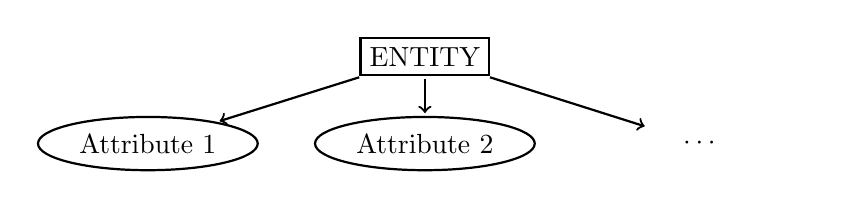
\begin{tikzpicture}[->, thick, shorten >=1pt, shorten <=1pt]
		\matrix [column sep=7mm, row sep=5mm] {
			& \node (e) [draw, shape=rectangle] {ENTITY}; & \\
			\node (a1) [draw, shape=ellipse] {Attribute 1}; &
			\node (a2) [draw, shape=ellipse] {Attribute 2}; &
			\node (a3)                       {$\qquad\quad\cdots\quad\qquad$}; \\
		};
		\draw       (e) -- (a1);
		\draw       (e) -- (a2);
		\draw       (e) -- (a3);
		\end{tikzpicture}
		\caption{An entity-relationship diagram.}
		\label{fig:ea}
	\end{figure}
	
	 Figure~\ref{fig:bigjohn} shows a more concrete example of a graph taken from Johnson, Rosebrugh and Dampney~\cite{Johnson:2001:VUS:545538.545541} and slightly modified here. Note in it the injective functions. Intuitively, for example, the function {\sc specialist} \raisebox{-1pt}{\Large $ \rightarrowtail$} {\sc medical practitioner} may be read, ``each medical practitioner is at most one specialist'', which makes sense as a practitioner cannot be more than one person. On the other hand, the {\sc specialist} {$ \rightarrow$} {\sc specialisation} function does not impose an at-most-one \textit{cardinality constraint} as it is quite possible, ``a specialisation may have more than one specialist''\footnote{Actually, the relationships between entities are usually read in the direction of the arrow---for example, ``a {\sc specialist} is a {\sc medical practitioner}. I have avoided that here to make my discussion of the cardinalities clearer.}.
	
	\begin{figure}
		\centering
		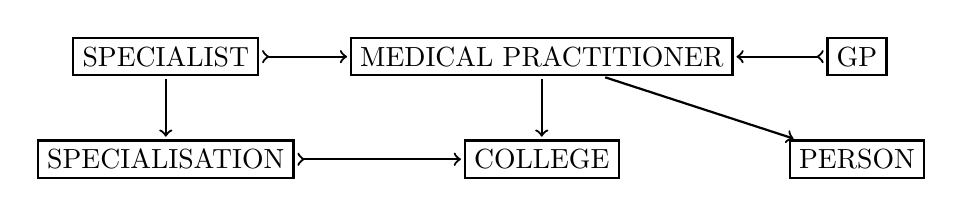
\begin{tikzpicture}[->, thick, shorten >=1pt, shorten <=1pt]
		\matrix [column sep=7mm, row sep=8mm] {
			\node (spst) [draw, shape=rectangle] {SPECIALIST}; &
			\node (prac) [draw, shape=rectangle] {MEDICAL PRACTITIONER}; &
			\node (gp) [draw, shape=rectangle] {GP}; \\
			\node (spon) [draw, shape=rectangle] {SPECIALISATION}; &
			\node (coll) [draw, shape=rectangle] {COLLEGE}; &
			\node (pers) [draw, shape=rectangle] {PERSON}; \\
		};
		\draw       (spst) -- (spon);
		\draw [>->] (spst) -- (prac);
		\draw [>->] (spon) -- (coll);
		\draw [>->] (gp)   -- (prac);
		\draw       (prac) -- (coll);
		\draw       (prac) -- (pers);
		\end{tikzpicture}
		\caption{Part of a graph for a health informatics database.}
		\label{fig:bigjohn}
	\end{figure}
	
	\subsection{Example: A File Sharing Website}
	Figure~\ref{fig:bigchris} shows a graph for a file sharing website. In it we see there are many {\sc user}s, who each are able to make multiple {\sc upload}s and {\sc comment}s. As well, many {\sc comment}s and Twitter-style {\sc hashtag}s can be made on {\sc upload}s. Unlike {\sc comment}s which are made by identifiable users, {\sc hashtag}s are not (unless it is a rule that they can only be left by the uploader, which is a constraint that is awkward to show using the ER model). An {\sc upload} can have many files.
	
	\begin{figure}
		\centering
		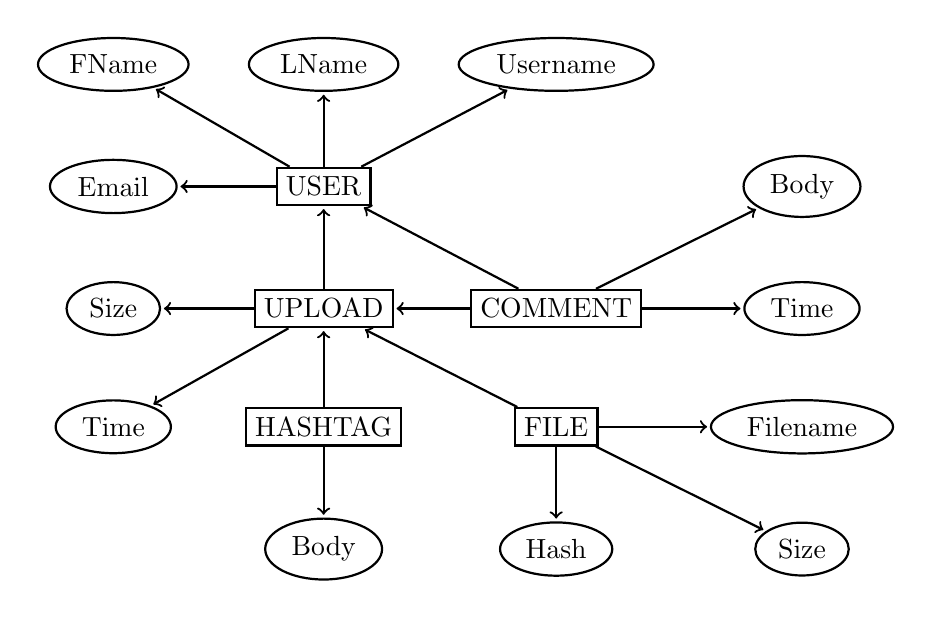
\begin{tikzpicture}[->, thick, shorten >=1pt]
		\matrix [column sep=7mm, row sep=8mm] {
			\node (fname) [draw, shape=ellipse] {FName}; &
			\node (lname) [draw, shape=ellipse] {LName}; &
			\node (username) [draw, shape=ellipse] {Username}; &
			\\
			\node (email) [draw, shape=ellipse] {Email}; &
			\node (euser) [draw, shape=rectangle] {USER}; &
			&
			\node (commentbody) [draw, shape=ellipse] {Body}; \\
			\node (uploadsize) [draw, shape=ellipse] {Size}; &
			\node (eupload) [draw, shape=rectangle] {UPLOAD}; &
			\node (ecomment) [draw, shape=rectangle] {COMMENT}; &
			\node (commenttime) [draw, shape=ellipse] {Time}; \\
			\node (uploadtime) [draw, shape=ellipse] {Time}; &
			\node (ehashtag) [draw, shape=rectangle] {HASHTAG}; &
			\node (efile) [draw, shape=rectangle] {FILE}; &
			\node (filename) [draw, shape=ellipse] {Filename}; \\
			&
			\node (hashtagbody) [draw, shape=ellipse] {Body}; &
			\node (hash) [draw, shape=ellipse] {Hash}; &
			\node (filesize) [draw, shape=ellipse] {Size}; \\
		};
		\draw       (euser) -- (fname);
		\draw       (euser) -- (lname);
		\draw       (euser) -- (email);
		\draw       (euser) -- (username);
		\draw       (eupload) -- (uploadtime);
		\draw       (eupload) -- (uploadsize);
		\draw       (ecomment) -- (commentbody);
		\draw       (ecomment) -- (commenttime);
		\draw       (ehashtag) -- (hashtagbody);
		\draw       (efile) -- (hash);
		\draw       (efile) -- (filename);
		\draw       (efile) -- (filesize);
		
		\draw       (eupload) -- (euser);
		\draw       (ecomment) -- (euser);
		\draw       (ecomment) -- (eupload);
		\draw       (ehashtag) -- (eupload);
		\draw       (efile) -- (eupload);
		\end{tikzpicture}
		\caption{An ER diagram for a (feature-impoverished) file sharing website.}
		\label{fig:bigchris}
	\end{figure}
	
	It is important to check that the functions used are appropriate. For instance, while a {\sc medical practitioner} can only be one {\sc specialist}, the injection {\sc comment} \raisebox{-1pt}{\Large $ \rightarrowtail$} {\sc user} would be inappropriate unless for some reason a user should make no more than one comment.
	
	Additionally, any parts of the graph which (do not) \textit{commute} should be carefully checked. A diagram is said to do so when the composites of the functions along two paths are necessarily equal. In this example there is what looks like a commuting diagram formed by the paths {\sc comment} {$ \rightarrow$} {\sc upload} {$ \rightarrow$} {\sc user} and {\sc comment} {$ \rightarrow$} {\sc user}. This is not a commuting diagram however because users are not restricted to commenting on their own uploads.
	
	Compare this to Figure~\ref{fig:bigjohn} where a {\sc specialist} is a {\sc medical practitioner} who is a {\sc member} of a {\sc college}, and a {\sc specialist} has a {\sc specialisation} which is a {\sc college}. In this case, the {\sc medical practitioner} and {\sc specialisation} must refer to the same {\sc college}, given a particular {\sc specialist}, so the diagram commutes.
	
	\section{Relational Databases}
	A relational database is one which uses a collection of tables to store and organise data. The name comes from the fact that data in a table is called a relation. This usage of this word is distinct from, but related to, the sense used in mathematics where, for example, a function is kind of relation.
	\subsection{Tables}
	A database's table is similar to one you might create in a spreadsheet, with a few possible differences:
	\begin{itemize}
		\item Data in the table is changed only by \verb|INSERT|, \verb|DELETE| and \verb|UPDATE| \textit{queries} (see Section~\ref{sec:sql}) which add, remove and change rows, respectively.
		\item Columns (attributes) cannot usually be easily added or removed once the database is implemented in software. Indeed, if this needs to be done, not enough time was spend designing the database.
		\item Rows must be unique.
	\end{itemize}
	
	To express an ER model as a table, one would consider each entity as a different table. The entity's attributes become the columns (or fields) of the table and rows symbolise instances of an entity. Functions between entities are encoded using primary keys and foreign keys:
	\begin{description}
		\item[Primary Key] This is one or more columns in the table used to uniquely identify rows. Often each row would be assigned an arbitrary integer.
		\item[Foreign Key] This is one or more columns containing the primary keys from another table.
	\end{description}
	Considering Figure~\ref{fig:bigjohn}, each {\sc person} would be given a primary key which would be included in the {\sc medical practitioner} table as a foreign key. The reason the keys would not be assigned the other way around is that the function needs to map from a {\sc medical practitioner} to a {\sc person}.
	\subsection{SQL} \label{sec:sql}
	SQL (Structured Query Language) allows users to view rows from tables using the \verb|SELECT| statement. \verb|INSERT|, \verb|DELETE| and \verb|UPDATE| operations are also possible (though these are not queries proper).
	
	Most SQL queries are of the following form
	\begin{lstlisting}[style=highlightable, frame=none, numbers=none, xleftmargin=0ex, xrightmargin=0ex, language=SQL]
SELECT column1, column2, ..., columnn FROM table1 WHERE constraints_here;
	\end{lstlisting}
	which would show the columns column1, column2---all the way up to columnn---from table1 which meet the given constraints (which are optional). An asterisk can be used in place of the columns to show all rows. For example, if the database represented by Figure~\ref{fig:bigjohn} was implemented, the query
	\begin{lstlisting}[style=highlightable, frame=none, numbers=none, xleftmargin=0ex, xrightmargin=0ex, language=SQL]
SELECT * FROM specialists;
	\end{lstlisting}
	would get every row from specialists, showing every column.
	
	\subsection{Example: The File Sharing Website Revisited}
	Now that I know something about relational databases, I can express the file sharing site as one. I am using MySQL as my DataBase Management System (DBMS), which can manage multiple databases simultaneously, so I need to explicitly create the database and give it a name:
	\begin{lstlisting}[style=highlightable, frame=none, numbers=none, xleftmargin=0ex, xrightmargin=0ex, language=SQL]
CREATE SCHEMA `filesharing_website` DEFAULT CHARACTER SET utf8 ;
	\end{lstlisting}
	Then the tables should be created. I will only show a few here starting with the {\sc user} table:
	\begin{lstlisting}[style=highlightable, frame=none, numbers=none, xleftmargin=0ex, xrightmargin=0ex, language=SQL]
CREATE TABLE `filesharing_website`.`user` (
	`username` VARCHAR(20) NOT NULL,
	`first_name` VARCHAR(45) NULL,
	`last_name` VARCHAR(100) NULL,
	`email` VARCHAR(256) NULL,
	PRIMARY KEY (`username`));
	\end{lstlisting}
	Now the {\sc upload} table is made:
	\begin{lstlisting}[style=highlightable, frame=none, numbers=none, xleftmargin=0ex, xrightmargin=0ex, language=SQL]
CREATE TABLE `filesharing_website`.`upload` (
	`idupload` INT NOT NULL,
	`fk_username` VARCHAR(20) NOT NULL,
	`time` DATETIME NOT NULL,
	`size` INT NOT NULL,
	PRIMARY KEY (`idupload`),
	INDEX `username_idx` (`fk_username` ASC),
	CONSTRAINT `username`
		FOREIGN KEY (`fk_username`)
		REFERENCES `filesharing_website`.`user` (`username`)
		ON DELETE NO ACTION
		ON UPDATE NO ACTION);
	\end{lstlisting}
	Notice that the \verb|idupload| field was not present in Figure~\ref{fig:bigchris}, but appears here. This primary key ensures each row can be uniquely identified. The \verb|fk_username| field was also added, which is a foreign key used to refer to a row in the {\sc user} table that allows us to say which user made the upload.
	
	The above SQL statements were generated automatically in MySQL Workbench, which is part of the reason lines like \verb|ON DELETE NO ACTION| can be seen. They refer to the fact that the DBMS can have \verb|DELETE| and \verb|UPDATE| operations \verb|CASCADE| changes through to other tables. If MySQL did not allow this, to delete a user account for instance would require all the following steps be done manually:
	\begin{enumerate}
		\item The corresponding row in the {\sc user} table is deleted.
		\item Any rows in the {\sc upload} table with a foreign key from the now deleted user must be deleted.
		\item Any rows in the {\sc comment} table with a foreign key from the now deleted user \textit{and} upload must both be deleted.
		\item The same is done for other tables with newly orphaned foreign key references.
	\end{enumerate}
	\subsubsection{Some Queries on The Database}
	A well-designed database should allow most queries to be expressed succinctly. It is then fitting that I test my new database with some queries. For example, \textit{how many uploads have a size greater than 10 megabytes?}
	\begin{lstlisting}[style=highlightable, frame=none, numbers=none, xleftmargin=0ex, xrightmargin=0ex]
mysql> select * from upload where size > 10*1024*1024;
+----------+-------------+---------------------+----------+
| idupload | fk_username | time                | size     |
+----------+-------------+---------------------+----------+
|        1 | dave42      | 2014-12-12 00:09:31 | 19975316 |
|        2 | dave42      | 2014-12-12 00:09:31 | 15254584 |
|        3 | dave42      | 2014-12-12 00:13:01 | 22986333 |
+----------+-------------+---------------------+----------+
3 rows in set (0.00 sec)
	\end{lstlisting}
	This answers my question reasonably well (assuming \verb|size| is measured in bytes), but I know I can do better as an {\sc upload} table with many entries poses a problem---the output from my above query would be too big to count manually. You might reasonably guess that the last \verb|idupload| shown is the number of rows, but this will probably not be true if one of the rows above it was deleted, because the IDs will not be automatically updated then. MySQL's aggregate function \verb|COUNT| can be used to solve this issue:
	\begin{lstlisting}[style=highlightable, frame=none, numbers=none, xleftmargin=0ex, xrightmargin=0ex]
mysql> SELECT COUNT(*) FROM upload WHERE size > 10*1024*1024;
+----------+
| COUNT(*) |
+----------+
|        3 |
+----------+
1 row in set (0.00 sec)
	\end{lstlisting}
	One thing which is apparent is that an SQL query will always return a table, even if the result is just a number.
	
	Now imagine that I am an elitist and that I habitually correct and criticise others' use of language so that I do not like users of my site writing the phrase ``YOLO''\footnote{This is an acronym meaning, ``you only live once'', from a song by rapper Drake. It gained infamy after being commonly used to justify extremely poor decisions.} in comments or using ``ur'' to mean ``your''. I would like to ask \textit{how many users' accounts should I delete?}
	\begin{figure}
	\begin{lstlisting}[language=SQL, caption={An example showing the use of nested queries, aggregate functions and SQL joins.}, label=lst:sqlbigboy]
SELECT	COUNT(*)
FROM
(
		SELECT	user.username
		FROM	user
		INNER JOIN
				upload
		ON		upload.fk_username = user.username
		INNER JOIN
				hashtag
		ON		hashtag.fk_idupload = upload.idupload
		WHERE	UPPER(hashtag.body) = 'YOLO'
		UNION
		SELECT	user.username
		FROM	user
		INNER JOIN
				comment
		ON		comment.fk_username = user.username
		WHERE	comment.body LIKE '% ur %'
)
	\end{lstlisting}
	\end{figure}
	What results is a fairly complicated query, however I would argue that this is not because of a poorly designed database as the question itself it complicated, consisting of two main parts: how many users made bad hashtags, and how many users wrote bad comments. Lines 4-12 and then 14-19 answer each of these respective questions in part, finding \textit{which} users performed the bad activities. Conceptually\footnote{A query may execute differently to the way it is written because of the \textit{query optimiser}, which can internally rewrite statements to improve performance.}, the \verb|UNION| keyword then combines the \verb|username|s from each of the resulting tables, creating a third one, which importantly does not have any \verb|username| repeated. The rows in this table are finally counted. One issue is that the query in Listing~\ref{lst:sqlbigboy} will not match instances of ``ur'' in comments unless they are surrounded by spaces.
	
	\subsection{Caveats with Multiple Concurrent Users}
	It is worth mentioning that when a database has multiple concurrent users, the same sorts of issues evoked in Chapter~\ref{ch:distributed} can occur---namely race conditions. This is an issue especially when multiple tables need to be modified to make the database consistent, like when deleting a {\sc user}. For this reason practical DBMSs need to be able to perform multiple queries as a single \textit{transaction} which can be \textit{rolled back} (undone) if it cannot be executed completely. While the transaction is being \textit{committed}, any resources involved (tables or rows) need to be \textit{locked} (the idea is the same as mutexes mentioned earlier) to prevent changes. This locking usually happens implicitly, though the user can manually request a lock.
	
	\chapter{Operating Systems}
	\section{Introduction}
	Modern Operating Systems (OSes) are extremely complicated things, managing a computer's hardware and software. To talk about an OS in its entirety in just the few pages I have here would be ambitious to say the least. Instead, I have a C program which hints at the underlying complexity of an OS while demonstrating important security concerns and the operation of the stack.
	
	\section{A Buffer Overflow Attack}
	Buffer overflow occurs when there are too much data for a \textit{buffer} (a region of memory) to store them, resulting in them \textit{overflowing} into an adjacent part of the memory.
	\subsection{Some Preliminaries}
	Computers deal with function calls using a \textit{call stack}, which is a last-in-first-out (LIFO) data structure that stores \textit{stack frames}, one containing the data associated with each function call. Stack frames can be added to or removed from only the top of the stack. This property makes it well-suited to coordinating calls, because the function which was last called should be the first to return.
	
	Inside each stack frame are the following, ordered from the higher in the stack to lower:
	\begin{itemize}
		\item Space for local variables.
		\item The return address, which is the memory location that the program should resume executing code from once the function has completed.
		\item Arguments passed to the function.
	\end{itemize}
	
	As an example, consider the code in Listing~\ref{lst:c}. When the \verb|do_work| function is called, the argument (a pointer) will be placed on the stack, then the return address (which roughly corresponds to line 29), followed by the array (line 6). The array is stored with the higher-indexed elements lower in the stack.
	
	\begin{figure}
	\begin{lstlisting}[language=C, label={lst:c}, caption={The C code of a program vulnerable to a buffer overflow attack.}]
#include <stdio.h>
#include <string.h>

void do_work (char * typed)
{
    char array[20];
    printf("What's on the stack?\n%p\n%p\n%p\n%p\n%p\n%p\n%p\n%p\n%p\n%p\n%p\n%p\n%p\n%p\n%p\n%p\n%p\n%p\n\n");
    strcpy(array, typed);
    printf("%s\n", array);
    printf("Now the stack looks like:\n%p\n%p\n%p\n%p\n%p\n%p\n%p\n%p\n%p\n%p\n%p\n%p\n%p\n%p\n%p\n%p\n%p\n%p\n\n");
}

void never_called (void)
{
    printf("how could I be executing?\n");
}

int main (int argc, char * argv[])
{
    printf("Where are my functions?\n");
    printf("do_work is at %p\n", do_work);
    printf("never_called is at %p\n", never_called);
    printf("main is at %p\n", main);
    if (argc != 2) {
        printf("usage: name string \n");
        return -1;
    }
    do_work(argv[1]);
}
	\end{lstlisting}
	\end{figure}
	\subsection{The Attack}
	If a program has a buffer which can overflow, (part of) the running instance of it can be modified. In this case, the return address in \verb|do_work|'s stack frame can be changed to redirect to \verb|never_called|. This attack is of such concern that most modern (circa post-2005) operating systems and compilers have features built in to prevent them.\footnote{These include Address Space Layout Randomization (ASLR) and canaries, which were briefly mentioned in class. On my machine, the exploit discussed here did not require these features to be disabled.} In any case, upon running the code in Listing~\ref{lst:c}, I received the following output:
	\begin{lstlisting}[style=highlightable, frame=none, numbers=none, xleftmargin=0ex, xrightmargin=0ex]
[139]christian@christian-pc /tmp $ ./a.out 0123456789
Where are my functions?
do_work is at 0x40058d
never_called is at 0x4005d8
main is at 0x4005e8
What's on the stack?
0x7fffffec
0x7ffff7dd77f0
0x13
0x6
0x7ffff7dd46a0
0x7ffff7dd77f0
0x7fffffffe595
0x4007ec
0xffffffff
(nil)
0x7ffff7ffe1e8
0x7fffffffe1c0
0x400667
0x7fffffffe2a8
0x200000000
(nil)
0x7ffff7a50995
(nil)

0123456789
Now the stack looks like:
0x7ffff7ff7000
0x7ffff7dd77f0
0xffffffffffffffff
0x7ffff7dd77f0
0x7ffff7dd46a0
0x7ffff7dd77f0
0x7fffffffe595
0x3736353433323130
0xff003938
(nil)
0x7ffff7ffe1e8
0x7fffffffe1c0
0x400667
0x7fffffffe2a8
0x200000000
(nil)
0x7ffff7a50995
(nil)
	\end{lstlisting}
	I noted a return address of \verb|0x400667|, which I needed to change to \verb|0x4005d8|. Now, running
	\begin{lstlisting}[style=highlightable, frame=none, numbers=none, xleftmargin=0ex, xrightmargin=0ex]
./a.out 0123456789012345678901234567890123456789$(cat a.bin)
	\end{lstlisting}
	in the terminal (where \verb|a.bin| is a binary file containing \verb|0xd80540|) modified the address appropriately, however I did expect to require only 20 characters (the number of elements in the array) of padding before the address instead of 40. Moreover, changing the size of \verb|array| by only a small amount did not usually result in me requiring more or less padding. Presumably this had something to do with alignment of data structures in memory and/or the size of the assembler instructions, however I did not have time to investigate.
	
	If the program had been written in a safer, higher-level language like Java, it would (probably) not have been vulnerable to this kind of attack.
	
	\chapter{This Week in The News}
	The ICT industry is new, complex and rapidly changing. As a software engineer, I will be expected to provide special skills and advice in this industry. It is therefore appropriate that I remain up-to-date with associated developments. This chapter is a collection of software engineering-related news that occurred during this semester, along with comments on their socio-technical relevance.
	
	\section{Primary Students Learn to Program}
	\textit{25 March.} Key points~\cite{news4}:
	\begin{itemize}
		\item Representatives from Sydney University, the Westpac Banking Group and Telstra have held talks with Education Minister Christopher Pyne and Communications Minister Malcolm Turnbull to provide funding ideas on how to train teachers in programming.
		\item 23,500 teachers would need training to introduce the new curriculum at a cost of \$23 million.
		\item NSW could have the new curriculum taught by 2017 at the earliest.
		\item Advanced programming will be an elective subject in Years 9 and 10 in Australia.
		\item Britain is making computer coding compulsory in all primary schools in September.
	\end{itemize}
	
	\subsection{Comments}
	It is in the best interests of industry to have a large, highly skilled workforce at their disposal. Robust software and good-quality, professional colleagues are what I would like as a software engineer as well. However, one possible issue with teaching programming at a primary-school level is job market saturation, which could devalue the work of good programmers.
	
	Now, software engineers are not programmers; the latter do not necessarily take a disciplined, methodical approach to creating software. However there is significant enough overlap in the two areas to be concerned about the future of Australia's ICT job market. One of the many roles of professional societies is to ensure fair pay.
	
	\section{UK Report Finds Cost of Data Breaches Doubled}
	\textit{29 April.} Key points~\cite{news7}:
	\begin{itemize}
		\item Though the number of companies hit by information security breaches was down on the previous 12 months, the PriceWaterhouseCoopers survey found that the severity and impact of attacks has increased.
		\item The average cost of the worst cyber security breach for big companies was between \$1.1 million and \$2.2 million, up from the 2013 survey.
		\item Cyber attacks on companies in Europe and the United States have increased in regularity and severity in recent years as "hacktivists" and criminals become increasingly sophisticated, requiring businesses to strengthen their defences.
		\item In spite of this, the survey found that 81 percent of big companies suffered a security breach in the past 12 months, down from 86 percent in the 2013 study. It also found most companies had increased their spending on IT security.
	\end{itemize}
	
	\subsection{Comments}
	The 80\% figure on security breaches is concerning. In banks and infrastructure (e.g. energy and transport) such a breach could cost anywhere from millions to lives. Software engineering then has far-reaching ethical implications.
	
	As well as the responsibilities of industry the story also highlights that society is changing. The fact that activism by hacking (``hacktivism'') has a name suggests that many not-necessarily-good people are becoming more technologically literate, and therefore increasing the frequency and severity of security breaches.
	
	It is therefore important for me to follow software engineering best practice principles and encourage my colleagues to do the same.
	
	\section{Software Bug Disrupts E-vote Count in Belgian Election}
	\textit{26 May.} Key points~\cite{news11}:
	\begin{itemize}
		\item A bug in an e-voting application halted the release of European, federal and regional election results in Belgium, the country's interior ministry said Monday.
		\item The fault appeared in the system despite the fact that the application was especially developed for these elections, was ``tested thousands of times'' and was certified by PriceWaterhouseCoopers, he said.
		\item Kommer Kleijn, spokesman for VoorEVA.be, a Belgian organization that rejects the e-voting system because ``it deprives voters from effectively verifying the elections in which they partake'' called the problems ``a catastrophe.'' ``They claim that the recording of the votes was done flawlessly, but who can verify that? We can't,'' Kleijn said.
		\item In Germany, the Federal Constitutional Court banned the use of electronic voting machines in 2009 because results from the machines were not verifiable. The Netherlands banned the practice in 2008 after a group of activists successfully demonstrated that  electronic voting machines then in use could be tampered with.
	\end{itemize}
	\subsection{Comments}
	It is difficult to say if e-vote system could have been improved by better software engineering techniques. If the Secure Embedded L4 (seL4) microkernel\footnote{\url{http://ssrg.nicta.com.au/projects/seL4/}} can be mathematically proven, why can the voting system not be verified and validated with the same degree of rigour?
	
	\chapter*{Postface (Self-Evaluation)}
	Part of being a professional involves evaluating one's conduct so that it can be improved where necessary. Throughout ELEC436, I feel that I have been a decent student, but there are areas I could improve upon. For instance, I have not been very vocal during class discussions. In the workplace I will not be reprimanded if I do this. Rather, I will likely go unnoticed and fail to thrive in my profession.
	
	About this report in particular, I think I have not shown very good time management---Chapter~\ref{ch:networking} is 18 pages long, but no other chapter is more than 8 pages. A Gantt chart or some kind of agenda would have been useful but limited as, to thoroughly plan the research portions of this report, I would already require a working knowledge of the fields.
	
	Additionally, I have not discussed professional societies or the expectations of the ACS-ES Join Board enough. 
	
	Otherwise, my technical knowledge is good. Perhaps, once marks have been deducted for the above shortcomings, my work amounts to a low-to-mid-range distinction.
	
	\bibliographystyle{unsrt}
	\bibliography{doc}
\end{document}